\subsection{Motor}\label{subsubsec:Motor}

Als Motor wird ein bürstenloser Gleichstrommotor (BLDC-Motor) verwendet. Diese Bauform wurde vom betreuenden Dozent vorgegeben.
Ein BLDC-Motor zeichnet sich dadurch aus, dass er zu den Antrieben mit dem besten Verhältnis zwischen Leistung und Gewicht zählt. Ausserdem verfügt er über ein relativ hohes Drehmoment. Die Anwendung bringt bis auf die Drehlager keinen Verschleiss mit sich. Er ist zuverlässiger, effizienter und zudem noch leiser als herkömmliche Motoren \cite{imajey_consulting_engineers_pvt_ltd_brushless_nodate}. Im folgenden Kapitel soll gezeigt werden, wie solch ein Motor aufgebaut ist und nach welchem Funktionsprinzip er funktioniert.

\subsubsection{Aufbau}\mbox{}\\

Ein bürstenloser Gleichstrommotor funktioniert im Grunde nicht nach dem Prinzip eines Gleichstrommotors. Vom Aufbau her ist er gebaut wie ein Wechselstrom-Synchronmotor, wobei die Erregung mit Permanentmagneten gewährleistet wird. Beim Synchronmotor am 400V-Netz geschieht die magnetisierung der Spulen mit der sinusförmigen Netzfrequenz. Beim BLDC-Motor hingegen über die wechselnde magnetisierung mit einem Gleichstrom. Es wird folglich eine Steuerlogik benötigt, welche diesen Gleichstrom auf die Spulen schaltet. In Abbildung \ref{fig:Aufbau_Synchron_und_BLDC} wird der Aufbau beider Motoren veranschaulicht. \cite{noauthor_burstenloser_2019}

\begin{figure}[h!]
\centering
\hspace{3cm}
\subcaptionbox{3-Phasen-Synchronmotor \cite{noauthor_difference_nodate}}{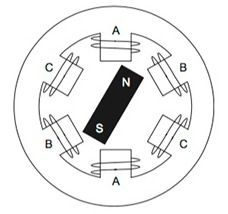
\includegraphics[height=4.5cm]{graphics/3_Phasen_Synchronmotor.jpg}}%
\hfill
\subcaptionbox{BLDC-Motor\cite{noauthor_choosing_2018}}{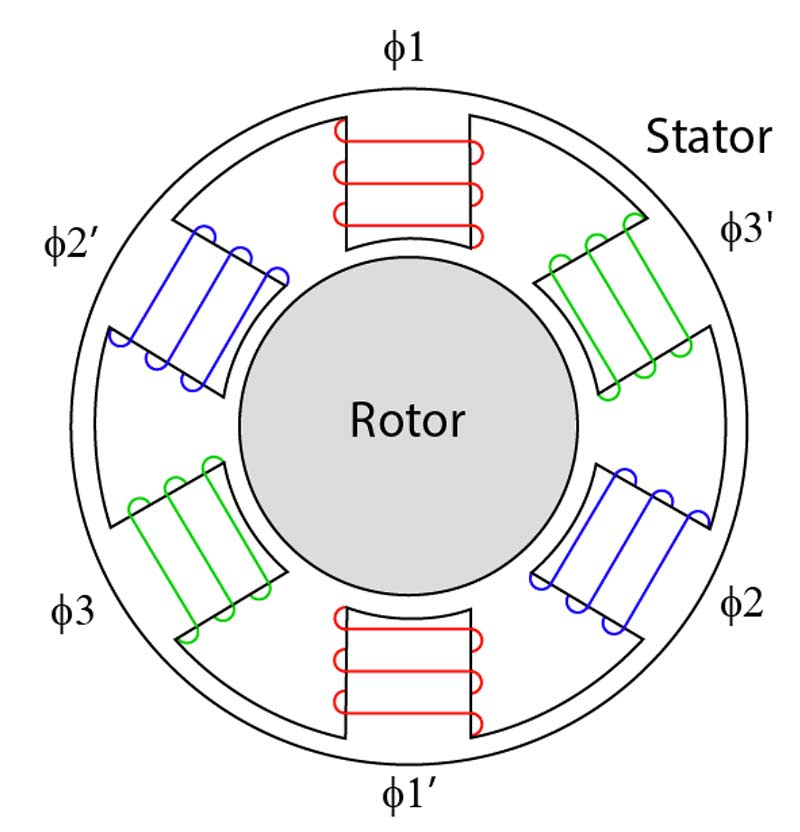
\includegraphics[height=4.5cm]{graphics/BLDC_Motor.jpg}}%
\hfill
\hspace{3cm}
\caption{Vergleich des Aufbaus zwischen Synchron- und BLCD-Motor.}
\label{fig:Aufbau_Synchron_und_BLDC}
\end{figure}

Hauptsächlich unterscheiden sich die BLDC-Motoren in Aussen- und Innenläufer.

\begin{tabbing}
\parbox[t]{.25\textwidth}{Aussenläufer} \= \parbox[t]{.75\textwidth}{Aussenläufer haben den Rotor ausserhalb des Stators (siehe Abb. \ref{fig:Kraftwirkung_BLDC_1}). Der Rotor bei Aussenläufern weist deshalb eine grössere Massenträgheit auf. Aus diesem Grund sind sie bevorzugt, wenn es darum geht zu erwartende Schwankungen in der Drehzahl oder im Drehmoment auszugleichen. \cite{bruner_burstenloser_2016} \cite{hembach_systematischer_2007}}\\
\\
\parbox[t]{.25\textwidth}{Innenläufer} \>\parbox[t]{.75\textwidth}{Innenläufer haben den Rotor auf der Innenseite des Stators (siehe Abb. \ref{fig:Aufbau_Synchron_und_BLDC}). Sie werden aufgrud der niedrigeren Trägheit für schnelle Richtugsänderungen bevorzugt.}
\end{tabbing}
\newpage
\subsubsection{Funktionsprinzip}

In Abbildung \ref{fig:Kraftwirkung_BLDC_1} sind die Spulen in der mitte statisch und bilden den Stator. Die Permanentmagnete sind am schwarzen Teil befestigt, welcher den Rotor darstellt. Durch die von einem Strom verursachte Magnetisierung der B-Spule ganz links auf der Abbildung, wird der Nord- und Südpol des Rotors im Gegenuhrzeigersinn angezogen. Die Kräftewirkung ist in der Abbildung mit einem grünen Pfeil dargestellt. Der Rotor beginnt sich zu drehen. Sobald der Rotor die Position erreicht, wie sie in der Mitte der Abbildung dargestellt wird, ändert sich die Magnetisierung von Spule B auf Spule C. Der Prozess der Anziehung und Drehung findet erneut statt und endet mit Erreichen der nächsten Position. Darauf folgt eine weitere Änderung der Magnetisierung von Spule C auf A. Wird dieser Prozess kontinuierlich wiederholt, dreht sich der Motor im Kreis.

\begin{figure}[h!]
	\centering
	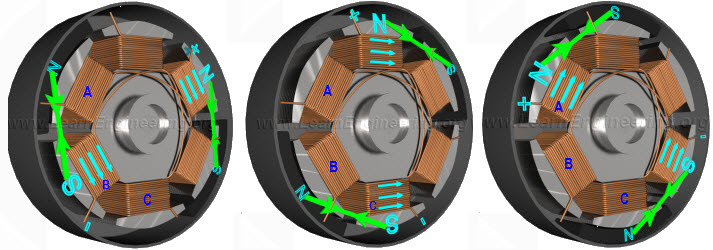
\includegraphics[height=4cm]{graphics/BLDC_Kraftwirkung_1.jpg}
	\caption{Kraftwirkung nur mit Anziehung (grün) \cite{imajey_consulting_engineers_pvt_ltd_brushless_nodate}}
	\label{fig:Kraftwirkung_BLDC_1}
\end{figure}

Würde man den Motor blockartig betreiben, hätte man nur wenige Positionen, welche angesteuert werden können. Zusätzlich können Vibrationen auftreten. Um dies zu verhindern werden die Spulen mit einem PWM-Signal gespiesen. Dies hat zur Folge, dass der Strom durch die Spulen und somit auch die Magnetisierung regulierbar ist. So kann der Motor mit feinen Positionsänderungen angesteuert werden und er verhält sich ruhiger im Betrieb. Das PWM-Signal kann beispielsweise wie in Abbildung \ref{fig:Motor_Kommuntierung_1} dargestellt generiert werden.

\begin{figure}[h!]
	\centering
	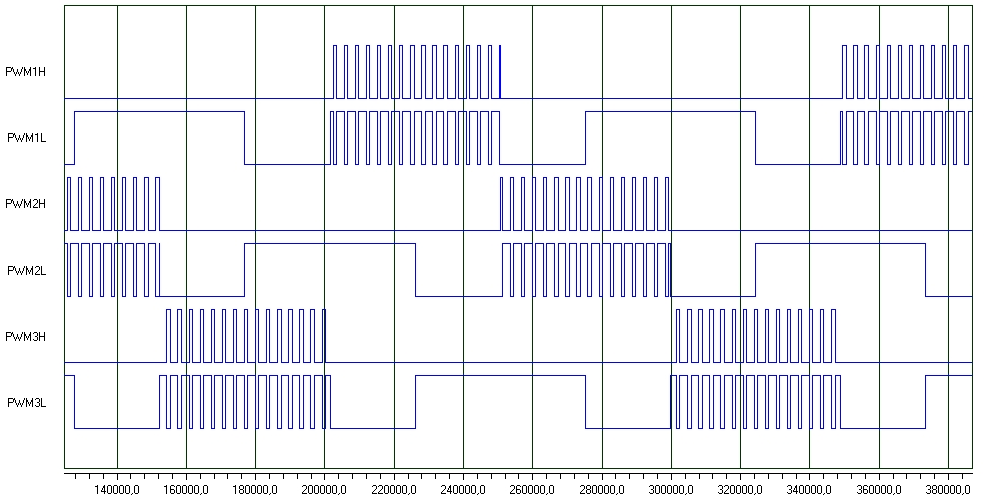
\includegraphics[width=0.8\textwidth]{graphics/Kommuntierung_BLDC_Blockkommuntierung.png}
	\caption{PWM-Signal der Kommuntierung. Das invers-PWM auf der Low-Side  wird geschaltet, um die Body-Diode zu entlasten.
	\cite{marc_bldc_2015}
	}
	\label{fig:Motor_Kommuntierung_1}
\end{figure}
\newpage
Die PWM-förmige Kommuntierungsspannung beeinflusst den Strom und somit die Magnetisierung der Spulen. Wird ein zunehmend breiteres PWM-Signal angelegt (grösserer Duty-Cycle), steigt der Strom. Wird das Signal wieder schmaler (kleinerer Duty-Cycle), sinkt der Strom. Dies ist in Abbildung \ref{fig:Motor_Kommuntierung_2} ersichtlich.

\begin{figure}[h!]
	\centering
	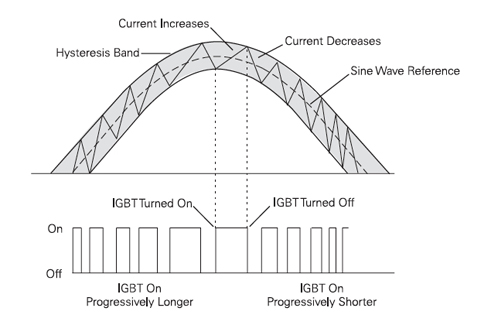
\includegraphics[width=0.8\textwidth]{graphics/Kommuntierung_BLDC_Sinus_Strom.png}
	\caption{Kraftwirkung nur mit Anziehung (grün) 
	\cite{lehane_wie_2012}
	}
	\label{fig:Motor_Kommuntierung_2}
\end{figure}
%\begin{figure}[h!]
%\centering
%\subcaptionbox{Ausgangssignal des PWM-Pins beim Einschaltvorgang.}{	\includegraphics[width=0.45\textwidth]{graphics/}}
%\hfill
%\subcaptionbox{Ausgangssignal des PWM-Pins beim Ausschaltvorgang.\label{fig:Motor_Kommuntierung_1}}{	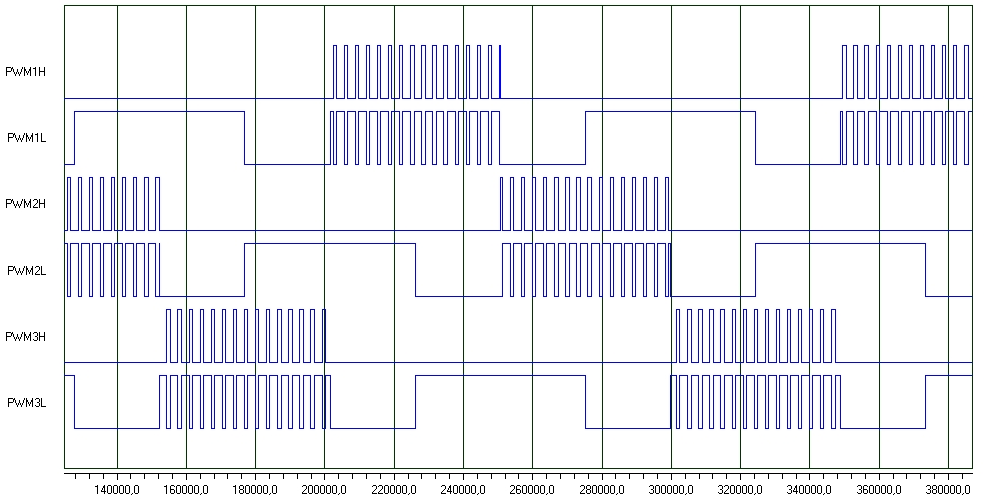
\includegraphics[width=0.45\textwidth]{graphics/Kommuntierung_BLDC_Blockkommuntierung.png}}
%\hfill
%\caption{Schematische und grafische Darstellung eines Resolvers.}
%\label{fig:Motor_Kommuntierung}
%\end{figure}

Dieser Prozess kann verstärkt werden, indem das Prinzip der Abstossung genutzt wird. Dazu werden zusätzlich die Spulen gemäss Abbildung \ref{fig:Kraftwirkung_BLDC_2} magnetisiert. Je nach Anwendung kann es aber auch möglich sein, dass man einen Rotor still halten möchte. Dazu lässt man die Spulen permanent magnetisiert, ohne das Feld zu ändern. Die Aufgabe, dies zu steuern, übernimmt der von Trinamic entwickelte TMC4672. Dessen Funktion wird in Kapitel \ref{subsec:TMC4671_EVAL_Boad} erläutert. 

\begin{figure}[h!]
	\centering
	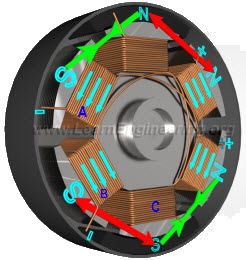
\includegraphics[height=4cm]{graphics/BLDC_Kraftwirkung_2.jpg}
	\caption{Kraftwirkung mit Anziehung (grün) und Abstossung (rot) \cite{imajey_consulting_engineers_pvt_ltd_brushless_nodate}}
	\label{fig:Kraftwirkung_BLDC_2}
\end{figure}

%Der Rotor wird foglich vom Stator ständig hinterhergezogen bzw. vorangetrieben. Mit der richtigen Ansteuerung wollen wir deshalb erreichen, dass wie in Abbildung \ref{fig:Kraftwirkung_BLDC_3} dargestellt, der Rotor wie ein Esel dem magnetischen Fluss (magnetic flux) hinterher rennt.
%
%\begin{figure}[h!]
%	\centering
%	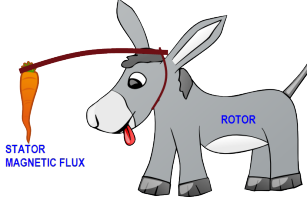
\includegraphics[height=3.5cm]{graphics/BLDC_Kraftwirkung_Esel.png}
%	\caption{Veranschaulichung Kraftwirkung \cite{imajey_consulting_engineers_pvt_ltd_brushless_nodate}}
%	\label{fig:Kraftwirkung_BLDC_3}
%\end{figure}

%\paragraph{Kommuntierung}\mbox{}\\

%Damit der Rotor der Magnetisierung nachrennen kann, braucht es ein sich änderndes Magnetfeld. In Abbildung \ref{fig:Kommuntierung_BLDC_1} wird dargestellt, wie die magnetisierung des Synchronmotors (links) und des BLDC-Motors (rechts) aussieht. Diese Aufgabe übernimmt der von Trinamic entwickelte TMC4672. Dessen Funktion wird in Kapitel \ref{subsubsec:TMC4671_EVAL_Boad} beschrieben.

%\begin{figure}[h!]
%	\centering
%	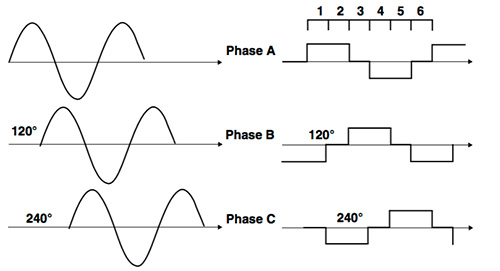
\includegraphics[height=4cm]{graphics/Sinus_und_Viereck_Signal.jpg}
%	\caption{Vergleich magnetisierung Synchronmotor und BLDC-Motor. \cite{noauthor_difference_nodate}}
%	\label{fig:Kommuntierung_BLDC_1}
%\end{figure}

%Abbildung \ref{fig:Aufbau_Synchron_und_BLDC} zeigt nochmals, dass der Synchronmotor direkt ans AC-Netz angeschlossen werden kann, während der theoretischen Aufbau für den DC-Motor noch einige komponenten benötigt.
%
%\begin{figure}[h!]
%\centering
%\subcaptionbox{3-Phasen-Synchronmotor am AC-Netz \cite{noauthor_synchronmotor_nodate}.}{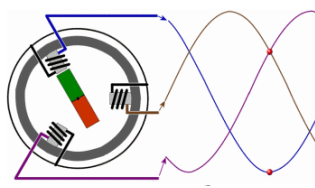
\includegraphics[height=4cm]{graphics/Synchronmotor.png}}%
%\hfill
%\subcaptionbox{BLDC-Motor am DC-Netz\cite{noauthor_choosing_2018}}{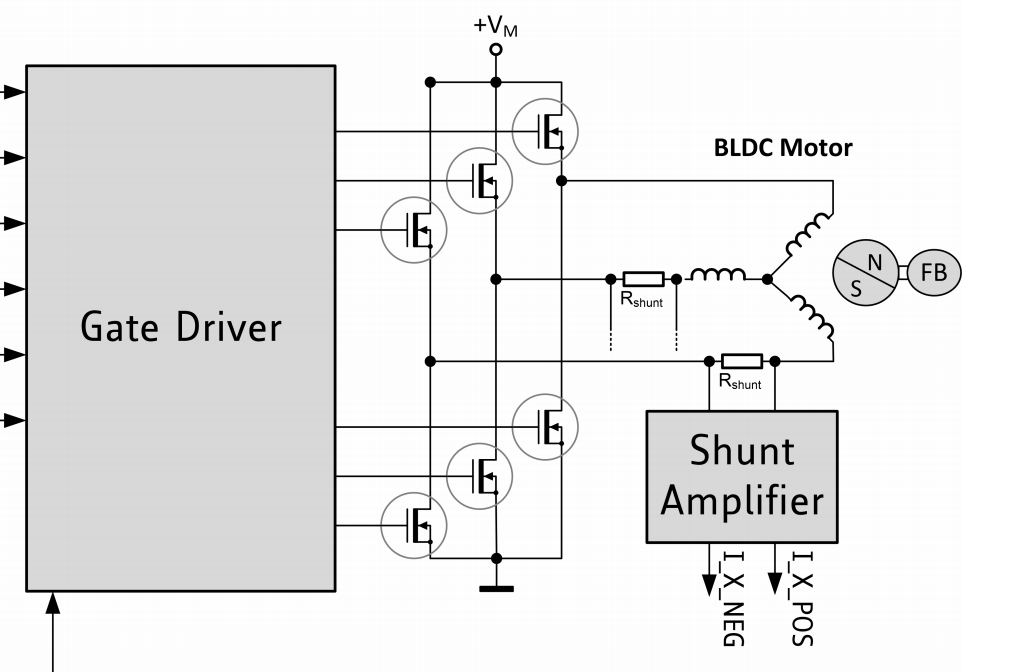
\includegraphics[height=4cm]{graphics/H_Bruecke_BLDC.png}}%
%\hfill
%\caption{Vergleich des Aufbaus zwischen Synchron- und BLCD-Motor\cite{trinamic_datasheet_2018}.}
%\label{fig:Aufbau_Synchron_und_BLDC}
%\end{figure}

%\paragraph{Motor}\label{par:Anforderungen_Motor}\mbox{}\\
%Der Motor ist folglich mit dem angegebenen Treiber für das Projekt verwendbar. Der Motor an sich hat folgende Eigenschaften:
%\begin{tabbing}
%\parbox[t]{.25\textwidth}{Anschlussspannung} \= \parbox[t]{.75\textwidth}{48 V}\\
%\parbox[t]{.25\textwidth}{Nenndrehzahl} \= \parbox[t]{.75\textwidth}{1500 rpm}\\
%\parbox[t]{.25\textwidth}{Nennmoment} \= \parbox[t]{.75\textwidth}{0.85 Nm}\\
%\parbox[t]{.25\textwidth}{Nennleistung} \= \parbox[t]{.75\textwidth}{0.13 kW}\\
%\parbox[t]{.25\textwidth}{Stillstandstrom} \= \parbox[t]{.75\textwidth}{5.41 A}\\
%\parbox[t]{.25\textwidth}{Gebersystem} \= \parbox[t]{.75\textwidth}{Resolver}\\
%\parbox[t]{.25\textwidth}{Bremse} \= \parbox[t]{.75\textwidth}{Nein}\\
%\parbox[t]{.25\textwidth}{Wellentyp} \= \parbox[t]{.75\textwidth}{Glatte Welle}\\
%\parbox[t]{.25\textwidth}{Anschluss} \= \parbox[t]{.75\textwidth}{2 SpeedTec Ready M23 Stecker, auf Motor montiert}\\
%\end{tabbing}